\chapter{Application Development}
\label{ch:application-development}

\section{Overview of the Application}

The application is designed to parse textual input that represents a cause-effect graph, converting it into both a visual and logical format. Upon execution, the system performs two key tasks:

\begin{itemize}
    \item \textbf{Graph Visualization}: The first task is to generate a visualized cause-effect graph from the provided textual input. This allows users to clearly see the logical dependencies between causes (inputs) and effects (outputs), facilitating easy analysis of the business logic. Visual validation of the graph is also possible.
    \item \textbf{Logical Transformation and Decision Table Generation}: In the second phase, the system transforms the cause-effect graph into a logical structure. Through a series of transformation steps, the graph is converted into Boolean logic, and ultimately a decision table is created. This decision table serves as a clear representation of the different logical conditions and their outcomes.
\end{itemize}

All results, including the visual graph, logical transformations, and decision table, are presented in the application's client interface, providing users with an intuitive and comprehensive view of the entire process. The application facilitates the creation of graphical models through a textual interface and displays the transformations leading to the output, which serves as the foundation for generating structured test cases in an optimized manner.

The goal of the application is to simplify and speed up the process of creating cause-effect graphs. Using a textual representation allows for a clearer and more precise definition of the graphs. This approach can effectively represent complex and nested business logic, accommodating various types of rules, causes, and effects.

\section{Technical Overview}

The application is built with a focus on efficiently parsing textual inputs, generating cause-effect graphs, and transforming them into logical structures and decision tables. Below is a detailed technical overview of the key components and technologies used in the development process.

\subsection{Technical Stack}

The application is built using a combination of modern technologies, ensuring scalability, maintainability, and ease of development. Below is the breakdown of the technical stack used across various layers of the application.

\subsubsection{Front-End (User Interface)}

The first layer, which is directly accessible to end-users, is the user interface or \emph{front-end}. In implementing this, I looked for a modern solution that could meet the application's requirements, providing flexibility and supporting rapid development in a well-structured, maintainable way.

Ultimately, I decided to go with \textbf{ReactJS} \cite{reactjs}, a popular \emph{JavaScript} based library, to build the web-based client application. \textbf{ReactJS} is a widely adopted library for developing user interfaces, particularly in single-page applications where data dynamically changes without requiring a full page reload.

But why \textbf{ReactJS}? \textbf{ReactJS} provides a component-based architecture that is highly modular and reusable, making it an excellent choice for building the dynamic and interactive elements of this application. \textbf{ReactJS} allows us to efficiently manage and update the user interface as users input data and the application generates and visualizes cause-effect graphs.

\textbf{ReactJS}'s strength is in its ability to create highly dynamic, performant, and modular user interfaces. For an application like this, which involves continuous interaction and visualization of cause-effect graphs, React is an excellent choice due to its component-based architecture and efficient handling of frequent updates. However, it does have a learning curve and often requires integrating third-party libraries for advanced features. Despite these challenges, its advantages make it a solid choice for building front-end applications.

\textbf{ReactJS} is a lightweight library on its own, so for more complex and structured solutions, additional tools and libraries are often required. For this project, several other libraries were essential to enhance functionality and streamline development. To align with modern styling principles, I integrated \textbf{Material-UI}, a design library that follows Google's Material Design guidelines, providing a clean and consistent user interface. Additionally, I used \textbf{SCSS} for styling, which offers a modular and maintainable approach to \textbf{CSS}, allowing for better organization and scalability as the application grows.

It's worth highlighting two key libraries that significantly contributed to the functionality of the editor and graph. For the editor, I utilized the Microsoft's \textbf{Monaco Editor}, a modern, lightweight, and highly configurable web-based code editor. This tool enhances user experience by providing helpful hints for structuring graphs. For visualizing the graphs, I integrated the \textbf{Dagre} library, which enables efficient graph rendering, arrangement and visualization.

\subsubsection{Back-End}

The next layer handles the business logic and provides functionality to the clients. For the back-end, I employed \textbf{Ktor}, a \textbf{Kotlin}-based framework designed for building asynchronous servers and web applications. \textbf{Ktor} is known for its flexibility and scalability, allowing developers to create robust \emph{API}s with minimal configuration. Its lightweight architecture makes it particularly well-suited for microservices and cloud-native applications. Additionally, \textbf{Ktor}'s seamless integration with \textbf{Kotlin}'s features, such as coroutines, enhances performance and responsiveness in handling concurrent requests. Overall, \textbf{Ktor} provides an efficient foundation for the back-end of the application, enabling smooth communication between the server and client.

The server's responsibilities include providing initialization data for the client, managing user requests, and executing graph scripts. \textbf{Kotlin} supports its own \emph{Domain-Specific Language} (DSL) implementation, which I utilized in the future development of the application. This \emph{DSL} serves as the backbone of the graphing language, allowing for more expressive and concise syntax when defining cause-effect relationships. By leveraging \textbf{Kotlin}'s \emph{DSL} capabilities, I was able to create a more intuitive interface for users to interact with the graphing functionality, enhancing the overall development experience and usability of the application.

For communication, the server is designed to respond via a \textbf{RESTful API} as well as through \textbf{WebSockets}. The \emph{RESTful API} facilitates standard \textbf{HTTP} requests, enabling seamless interactions between the client and server for data retrieval and manipulation. This allows clients to make synchronous calls for initialization data and other resources.

In addition, the \emph{WebSocket} implementation provides a persistent connection, enabling real-time communication between the client and server. This is primarily used to provide real-time support for the editor.

Currently, the application does not store any data, so there is no need for a connection to a database or any other external storage. Thus, the persistence layer is absent.

\subsubsection{Version Control and CI/CD}

I used \textbf{Git} as the version control system during the development process and \textbf{Microsoft Azure} as the remote server for version control. To enhance searchability, I linked an \textbf{Azure Board} to the repository and created various tasks. Each task's unique identifier is included in the \textbf{Git} commit messages, allowing the server to automatically associate them with the corresponding tasks. Additionally, I used feature branches for implementation and applied Pull Requests for these branches when it was ready to be merged into the main branch. Each request also identifies the connected tasks based on the commit messages.

I also leveraged the \textbf{Microsoft Azure Pipeline} feature to automate the deployment process. These pipelines are automation scripts that, with proper configuration, can automatically generate artifacts from pushed states. I created two pipelines for this project to help validate the correctness of the committed states and automatically generate distribution artifacts.

\begin{itemize}
	\item The first pipeline is dedicated to generating assembled documentation from \textbf{LaTeX}-formatted sources. This pipeline produces a PDF document as an artifact.
	\item The second pipeline focuses on building and packaging the application. It compiles the back-end using \textbf{Gradle} and the front-end using \textbf{Yarn} package manager. Once the build processes are complete, this pipeline packages the compiled front-end code into the back-end package and designates it as an artifact. Additionally, the compiled and built results are packaged into a \textbf{Docker} image with a pre-installed environment and published to the \textbf{Docker Hub} platform. This facilitates deployment in future steps.
\end{itemize}

\subsubsection{Deployment}

For deployment, I am utilizing \textbf{Docker} with a \emph{Linux-based} environment. \textbf{Docker} enables the application to be packaged and distributed in a way that ensures it can run independently of the underlying platform. This containerization simplifies the deployment process, allowing the application to maintain consistent behavior across various environments.

Why \textbf{Docker}? \textbf{Docker} is an open-source platform that automates the deployment, scaling, and management of applications within lightweight, portable containers. Each container encapsulates an application along with its dependencies, ensuring that it runs consistently across different computing environments, whether in development, testing, or production. \textbf{Docker} streamlines the application development lifecycle by allowing developers to package their applications in a standardized unit, facilitating easier deployment and scaling while minimizing compatibility issues.

The generated \textbf{Docker} images can be used to create containers that are ready for execution. Additionally, these containers assist in scaling performance and availability while preventing overload. With the aid of a \emph{load balancer} and \textbf{Kubernetes}, we can automatically increase the number of containers as needed.

\subsection{Application Architecture}

The architecture of the application is based on a straightforward two-layered model. As the name suggests, the application is divided into two layers: the Front-End and the Back-End. Further details on figure \ref{fig:app-arch}. 

\begin{figure}[H]
	\centering
	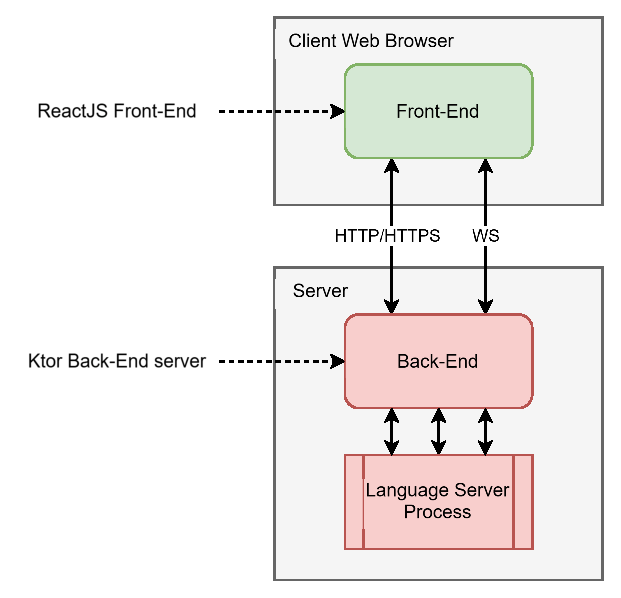
\includegraphics[width=0.5\textwidth,height=200px]{AppArch}
	\caption{Application Architecture}
	\label{fig:app-arch}
\end{figure}

\begin{compactitem}
    \item \textbf{Front-End layer}: This layer is responsible for the user interface and user experience. It handles the presentation of data and interactions with the users, providing a seamless and intuitive interface for creating and managing cause-effect graphs. It is highlighted in green in Figure \ref{fig:app-arch} and operates within the client's web browser.
    \item \textbf{Back-End layer}: This layer manages the application's business logic, data processing, and communication with the front-end. It handles requests from the client, processes them, and sends back the appropriate responses. It is highlighted in red in Figure \ref{fig:app-arch} and operates on a remote server.
\end{compactitem}

The communication between the two layers is bidirectional and can occur via either \emph{HTTP/HTTPS} or \emph{WebSocket} (WS) protocols. 

In the Figure \ref{fig:app-arch}, you can see that the server manages communication with multiple child processes that provide the functionalities of the \textbf{Kotlin Language Server}. Further details about the language server in the section \ref{sec:kotlin-language-server}.

\section{Implementation Details}

Upon accessing the server's address, the user is directed to the web front-end of the application via the index route. From this interface, the user can define a graph through the editor. Once the graph definition is completed and the execution is initiated, the source code is sent to the server for parsing and transformation. The server processes the input and returns the corresponding results, which are then displayed on the client interface.

For a more detailed description of the user interface and its features, see the next \ref{sec:ui} section.

\subsection{Parsing Graph Code}

The first step in the process is parsing the graph code. Once the source code arrives at the server, it is passed to the Kotlin Script parser engine. This engine parses the code and converts it into a Kotlin data model. The data model encapsulates the structure of the graph, including its nodes and relationships. After transforming the textual input, it evolves into this structured model, which can be utilized in subsequent processes.

The Kotlin Script engine can parse Kotlin code in a runtime environment and return the result. This is possible because the graph language is, in fact, a Kotlin Script. By leveraging Kotlin's DSL (Domain-Specific Language) structure, the language model was developed. The graph language itself consists of a series of Kotlin methods nested within each other, enabling flexible and dynamic representation of the cause-effect graph through executable Kotlin code.

Many Kotlin features enable the created language to be compact and easy to use. Features like extension functions, lambda expressions, and type inference make the syntax more concise, while Kotlin's strong typing system ensures robustness. These language constructs simplify both the definition and manipulation of the cause-effect graph, allowing for more readable and maintainable code.

\subsubsection{Graph Language Details}

In the code example \ref{src:basic-rule-def}, we see a basic rule definition. After importing the necessary packages, the definition begins with the \emph{graph} clause, which serves as the root of the language. Everything within the \emph{graph} block must consist of either rules or meta-cause data.

\lstset{caption={Definition of a basic rule for the graph}, label=src:basic-rule-def}
\begin{lstlisting}[language={Kotlin}]
import eu.karcags.ceg.graphmodel.dsl.*

graph {
	rule {
        cause("C1") { variable("a") + lit(1) eq lit(1000) }
        effect { "Access denied" }
    }
}
\end{lstlisting}

In \ref{src:basic-rule-def} example, only a single rule has been defined using the \emph{rule} clause. Each rule must contain at least one cause and one effect, which are created using the \emph{cause} and \emph{effect} clauses respectively.

The \emph{effect} clause contains a string value that represents the effect's description. For the \emph{cause}, we need to provide a predefined identifier, such as \textbf{"C1"} and the content must include an associated logical expression.

These expressions also follow a specific structural definition. Currently, each expression consists of a logical operator that connects two operands, forming a basic logical relationship between them.

\begin{compactitem}
	\item \textbf{Operators}: The operators follow standard logical conventions, consisting of six main types.
		\begin{compactitem}
			\item \textbf{Equivalence}: The \emph{eq} clause is used to define equivalence between two operands, establishing that both operands must be logically equal for the expression to hold true.
			\item \textbf{Inverse Equivalence}: The \emph{neq} clause serves as the inverse of the \emph{eq} clause, asserting that the expression is true when the two operands are not equal.
			\item \textbf{Lower than}: The \emph{lt} clause establishes a "less than" relationship between two operands. It is primarily used with numerical values.
			\item \textbf{Lower than or equal}: The \emph{lte} clause represents the "less than or equal to" operator and also allows for equivalence between the operands.
			\item \textbf{Greater than}: There is another side to these operators. The \emph{gt} operator signifies "greater than" and is primarily used with numeric operands.
			\item \textbf{Greater than or equal}: The counterpart of operator "greater than" is \emph{gte}, which extends the expression to include the equivalence as well.
		\end{compactitem}
	\item \textbf{Operands}:
		\begin{compactitem}
			\item \textbf{Literal}: For ease of use, a custom \emph{lit} clause has been introduced in place of standard Kotlin literals. This clause can contain constant values of various types, such as \textbf{Int}, \textbf{Double}, \textbf{Boolean}, and \textbf{String}, making the language more user-friendly and simplifying the expression of constant values within the graph definition. 
			\item \textbf{Variable}: For dynamic data, variables can be defined using the \emph{variable} clause. This requires only providing a valid variable name, which can then be used within the expressions, allowing for more flexible and dynamic rule definitions.
			\item \textbf{Expression}: The operand can also be a complex expression. By utilizing the four mathematical operations—addition (+), subtraction (-), multiplication (*), and division (/)—we can create expressions from simple operands, such as literals or variables.
		\end{compactitem}
\end{compactitem}

In the \ref{src:basic-rule-def} example, the expression for the \textbf{C1} cause represents a straightforward equivalence between the \emph{literal} 1000 and the sum of the \emph{variable} \textbf{a} and the \emph{literal} 1.

In the following example \ref{src:complex-rule-def}, we see three more complex rule definitions. By utilizing the repeated \emph{rule} clause, additional rule definitions can be incorporated.

A new cause type has been introduced in the updated graph definition. Unlike regular causes, which are defined within a rule, these are defined at the graph level, making them not directly connected to any specific rule by default. These are referred to as meta-causes. This feature allows users to reuse existing cause definitions across different rules, enhancing modularity and efficiency. Aside from these differences, the \emph{cause} clause functions in the same way as it does at the rule level.

In the third rule definition, there is an example of cause reuse. By utilizing the \emph{causeById} clause along with a unique name, the previously defined cause can be referenced. With this solution, all causes can be reused, but each cause can only be defined once.

\lstset{caption={Definition of a complex rules for the graph}, label=src:complex-rule-def}
\begin{lstlisting}[language={Kotlin}]
import eu.karcags.ceg.graphmodel.dsl.*

graph {
	cause("C1") { variable("a") lt lit(12) }
	rule {
        and {
            cause("C2") { variable("c") neq lit(1000) }
            not { cause("C3") { variable("b") eq variable("a") } }
        }
        effect { "Access is deined" }
    }
    rule {
        or {
            cause("C4") { lit(2.0) gt variable("c") }
            and {
                cause("C5") { lit(true) eq variable("d") }
                cause("C6") { lit(0) lte variable("a") }
            }
        }
        effect { "Access is granted" }
    }
    rule {
        causeById("C1")
        effect { "Access is granted with guest user" }
    }
}
\end{lstlisting}

Certainly, these basic causes alone are insufficient to construct complex business logic within the graph. Therefore, it's possible to encapsulate the \emph{cause} clauses within logical clauses such as \emph{or}, \emph{and}, or \emph{not}. These operators merely wrap the defined causes, allowing for more intricate relationships and logic.

In the \emph{not} clause, only a single child can be encapsulated, whereas the \emph{or} and \emph{and} clauses require at least two children. This distinction allows for different logical structures and complexity within the graph.

These logical clauses can be nested independently within each other; however, at the end of each logical tree, a cause definition must be present. This ensures that every logical expression ultimately relates back to a specific cause, maintaining the integrity of the graph structure.

In example \ref{src:complex-rule-def}, the first and second rule definitions illustrate a more complex business logic through the use of nested cause clauses. In the second rule, the cause is defined as an \textbf{OR} operation that includes the \textbf{C4} cause as one of its components, alongside an \textbf{AND} definition. Within this \textbf{AND} definition, two additional causes, \textbf{C5} and \textbf{C6}, are included. Together, these components form the overall cause for the rule, showcasing the flexibility of combining different logical structures to capture intricate business logic.

\subsection{Transform Into Visual Graph}

Once the source code is parsed, the resulting graph model serves as the foundation for subsequent processes and transformations. One of these processes involves generating a visual representation of the graph for Front-End visualization and display.

The process is straightforward. From the graph model, all visual nodes are identified. The node discovery is an uncomplicated procedure. First, the algorithm locates all effects in the model and converts them into graph nodes. Next, all causes are similarly transformed into graph nodes. The graph visualizes the logical relationships between these nodes, thus all logical connections among the cause nodes are also represented as graph nodes.

Alongside node detection, we also need to gather the edges for the graph. These edges represent the one-way arrow connections between the nodes. If a rule contains only one cause definition, the graph visualization for that rule will consist of two nodes connected by an arrow from the cause to the effect. However, if the cause involves a complex nested relation, the logical nodes created will be traversed as part of the rule's graph flow.

Let's examine an example. In the \ref{src:complex-rule-def} graph definition, the second rule will be visualized as shown in the following figure:

\begin{figure}[H]
	\centering
	\includegraphics[width=0.8\textwidth,height=140px]{ComplexGraphDefRule2}
	\caption{Visual graph representation of \ref{src:complex-rule-def} graph second rule definition}
	\label{fig:complex-graph-def-rule-2}
\end{figure}

The transformation result will yield a collection of independent nodes along with a set of edges, which include references for both the starting and ending points.

\subsection{Transfrom Into Logical Formulas}

The transformation involves a straightforward translation between the graph model and logical formulas, along with various logical formula refiners that perform modifications, optimizations, and simplifications.

\subsubsection{Translate Graph Model into Logical Formulas}

In the first step each rule in the graph is translated into logical definition pairs. The first element of the pair represents the destination effect, serving as a symbolic entry that corresponds to the second element, which is a combined logical definition. This definition is constructed from the rule's \emph{cause} clauses or the wrapping logical operator clauses. The transformation process is straightforward, with each clause representing its own logical definition. The \emph{and} clause will be represented as an \textbf{AND} object, while the \emph{cause} clause will simply become a standalone logical node.

Let's examine the first step in the previously mentioned example \ref{src:basic-rule-def}. The translation process for this single-rule graph is quite straightforward.

\begin{compactitem}
	\item $ E1 = C1 $
\end{compactitem}

The representation is straightforward, with an equivalence between \textbf{E1} and \textbf{C1}. However, all node metadata is stored in the underlying data model. To see a more complex result, let's examine the \ref{src:complex-rule-def} example.

\begin{compactitem}
	\item $ E1 = C2 \land \lnot C3 $
	\item $ E2 = C4 \lor (C5 \land C6) $
	\item $ E3 = C1 $
\end{compactitem}

In this case, there are three rules. The third rule is a simple equivalence between a cause and an effect, but the first two are more complex, involving nested structures with logical operators like \textbf{AND}, \textbf{OR}, and \textbf{NOT}. These operators combine multiple causes, making the resulting logical expressions more intricate.

\subsubsection{Refining of Logical Formulas}

The straightforward translation of the rules into logical formulas is insufficient for subsequent steps, such as decision table creation or test generation. Therefore, we need to further refine and modify these formulas to ensure they are usable in those processes. This includes simplification, normalization, and possibly restructuring the logic for better test coverage and decision-making accuracy.

In the application, the logical formula system undergoes a refiner pipeline, where each step in the pipeline modifies some aspect of the formula structure. These refiners apply transformations such as simplifications, optimizations, and logical normalizations. The output from one refiner serves as the input to the next, ensuring that by the end of the pipeline, the logical formula system is well-structured, optimized, and ready.

The list of the refiners:

\begin{itemize}
	\item \textbf{Negation Inward Mover}: The first element of the pipeline is responsible for pushing all negations inward within the logical definition. Using \textbf{De Morgan's law}, any negation is moved deeper into the structure, applying directly to the individual nodes. This process ensures that negations only appear at the operand level. Additionally, any duplicate or unnecessary negations are eliminated during this step, simplifying the overall structure of the formula.
	\item \textbf{Pre-Optimizer}: The second element of the pipeline focuses on optimizing the results of the first step by eliminating any unnecessary nodes. This step ensures that redundant components, such as statements that are always true or logically irrelevant elements, are removed or collapsed from the logical formula.
	\item \textbf{DNF}: The last element of the pipeline focuses on converting the logical formula into DNF. The algorithm processes all complex or convertible logical definitions, breaking them down into a full DNF, where the formula is expressed as a disjunction of conjunctions. Any simple logical definitions that are already in their simplest form are left unchanged, ensuring efficiency while maintaining the integrity of the logical structure.
\end{itemize}

\subsection{Construct Decision Table}

After passing through the pipeline of refinement steps, the logical formulas are fully optimized and ready for the conversion. This conversion process transforms the refined logical expressions into a structured table that clearly defines the relationships between various causes and their corresponding effects.

The optimized DNF rules are now ready to be translated into a Decision Table. The process involves individually constructing each logical definition into at least one column. For simple definitions, such as single-node conditions or basic \textbf{AND} operations, each is translated directly into a single column. This is because they can be expanded into a disjunction containing only one item.

After the DNF transformation, more complex items (those that are disjunctions of conjunctions) must be represented as multiple columns in the decision table. Each conjunction within the disjunction becomes a separate column, and all columns for a given rule will share the same effect.

For example, let's look at the second rule from the previous example and how it would appear in table format:

\begin{table}[H]
	\centering
	\begin{tabular}{ | m{0.12\textwidth} | m{0.12\textwidth} | m{0.12\textwidth} | m{0.12\textwidth} | m{0.12\textwidth} | }
		\hline
		\textbf{Nodes} & \textbf{Rule 1} & \textbf{Rule 2} & \textbf{Rule 3} & \textbf{Rule 4} \\
		\hline \hline
		\emph{C1} & - & - & - & 1 \\
		\hline
		\emph{C2} & 1 & - & - & - \\
		\hline
		\emph{C3} & 0 & - & - & - \\
		\hline
        \emph{C4} & - & 1 & - & - \\
		\hline
        \emph{C5} & - & - & 1 & - \\
		\hline
        \emph{C6} & - & - & 1 & - \\
		\hline \hline
        \emph{E1} & 1 &  &  &  \\
		\hline
		\emph{E2} &  & 1 & 1 &  \\
		\hline
		\emph{E3} &  &  &  & 1 \\
		\hline
	\end{tabular}
	\caption{The decision table of the \ref{src:complex-rule-def} graph definition}
	\label{tab:complex-graph-decision-table}
\end{table}

For the first and last graph rules, only a single column is needed in the decision table, as their logical structure is simple. However, the second graph rule requires two columns because its DNF form is a disjunction of two elements. Each element can cause the actiovation of the corresponding effect.

\section{User Interface}
\label{sec:ui}

The user interface of the application is designed to be simple and lightweight. It follows a single-page layout that effectively accommodates the main functionalities. The key features are organized in a tabbed format, with each feature residing in its own dedicated tab. This structure ensures that users can easily navigate between different functionalities without unnecessary complexity, enhancing the overall user experience.

\subsection{Editor}

By default, the \textbf{Editor} tab is selected, and all other tabs are disabled, as there is no valid graph definition present initially. The editor's starting value consists of only an import statement and a graph clause, providing a clean and minimalistic environment for users to begin defining their cause-effect graphs.

Below the editor, there is a message box that displays the results of each execution. It shows either successful execution messages or error responses.

Below the messages box, there are two buttons. The first button is the \textbf{Reset} button, which restores the editor's content to its initial state, regardless of any edits made. The second button is the \textbf{Execute} button, which is disabled by default. Once the user modifies the content in the editor, the \textbf{Execute} button becomes enabled and is ready for use.

When the \textbf{Execute} button is clicked, the client sends the editor content to the server for evaluation. If the execution encounters any errors, an error message will be displayed in the mentioned messages box, indicating the unsuccessful execution. In other cases, the system will parse the content and define the graph. Once the conversions are complete, the results will activate the other tabs, allowing users to access the newly generated information.

\begin{figure}[H]
	\centering
	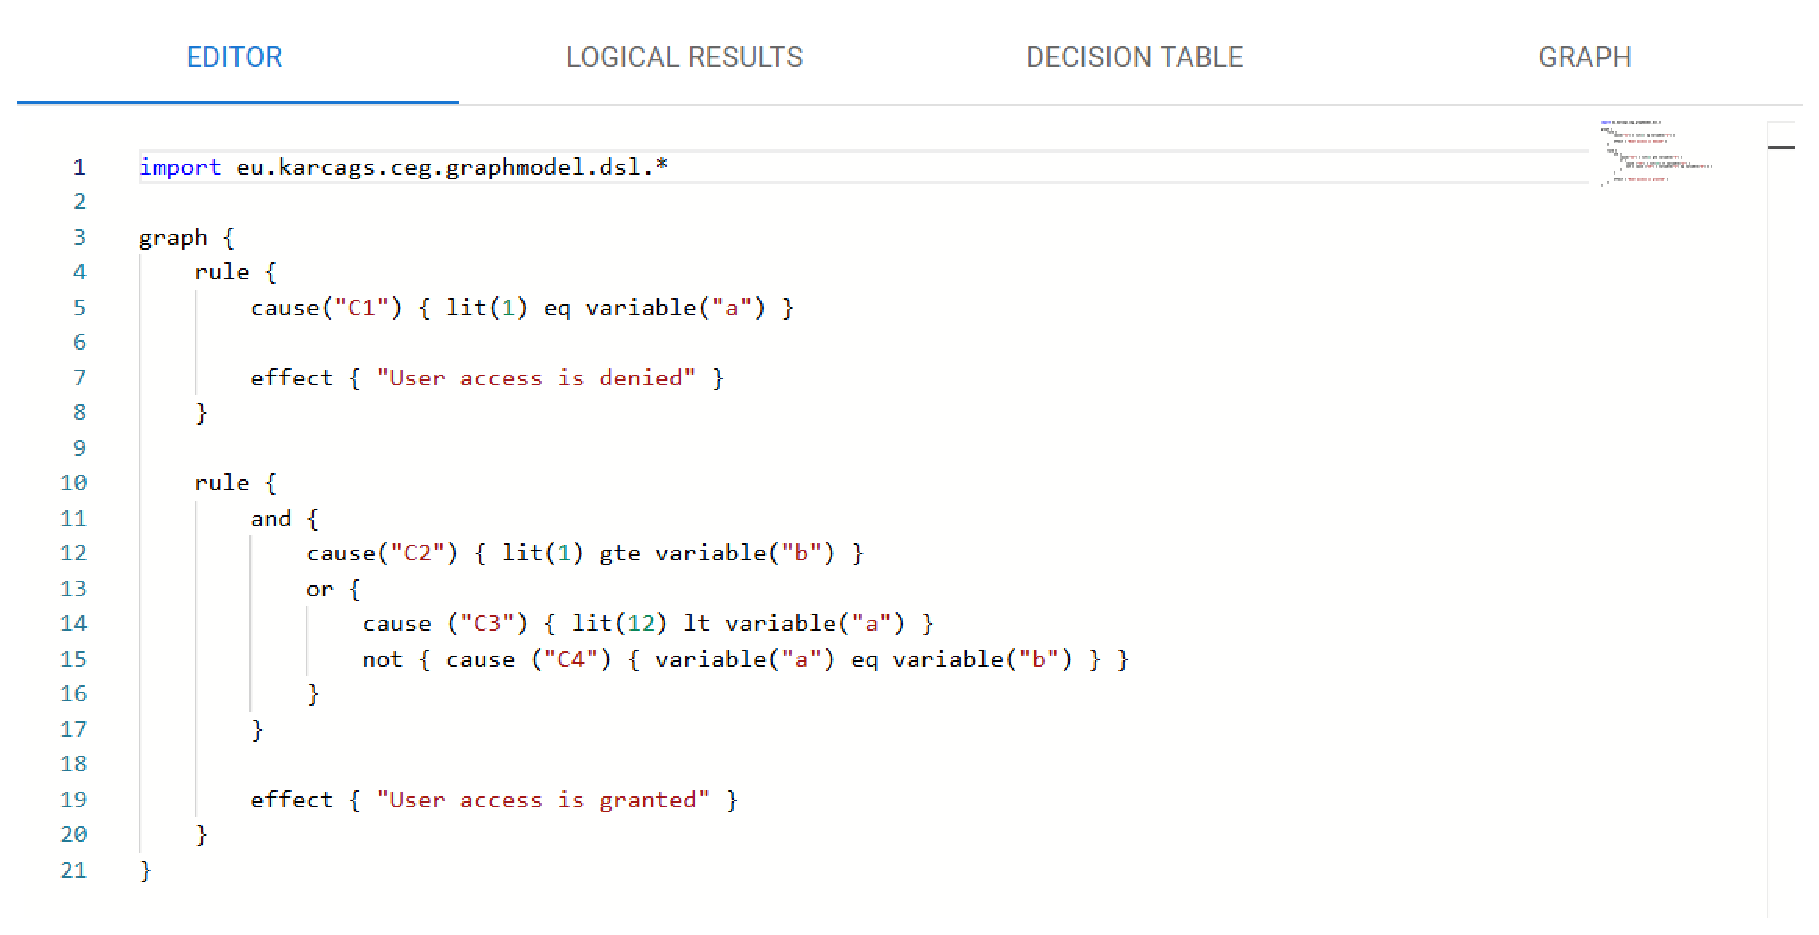
\includegraphics[width=0.8\textwidth,height=160px]{UIEditor}
	\caption{User Interface - Editor tab}
	\label{fig:ui-editor}
\end{figure}

The editor assists users by providing color coding and code IntelliSense features, which include helpful snippets. These enhancements improve the user experience by making it easier to write and understand the graph definitions, reducing the likelihood of errors and streamlining the overall editing process.

\subsection{Logical Results}

After a successful execution, the tabs that depend on the \textbf{Editor} will become available. The \textbf{Logical Results} tab displays the logical formulas parsed from the graph language, along with the corresponding logical formulas after the transformation steps. Each transformation step is presented for each rule, providing a clear overview of the progression from the initial graph to the final logical representation.

\begin{figure}[H]
	\centering
	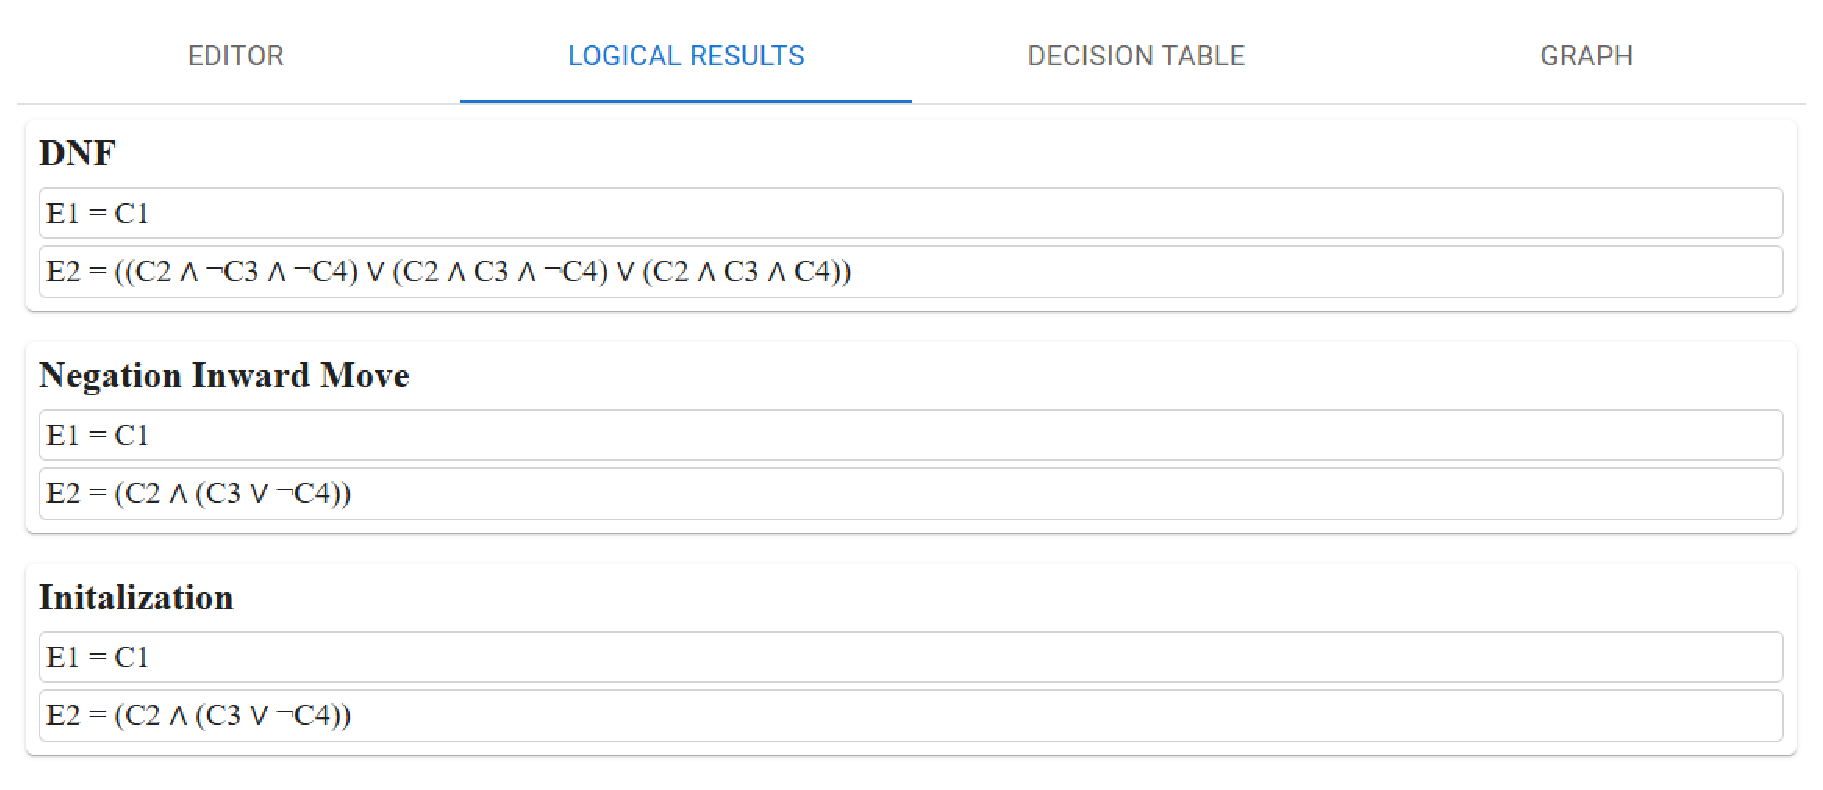
\includegraphics[width=0.8\textwidth,height=160px]{UILogicalResults}
	\caption{User Interface - Logical Results tab}
	\label{fig:ui-logical-results}
\end{figure}

\subsection{Decision Table}

From the final logical results, the system generates a decision table, which is displayed on the third tab. Each rule is converted into one or more columns in the table. Each column collects the causes and their corresponding values necessary to invoke a specific effect, providing a clear and organized representation of the decision-making logic for the further test generation process.

\begin{figure}[H]
	\centering
	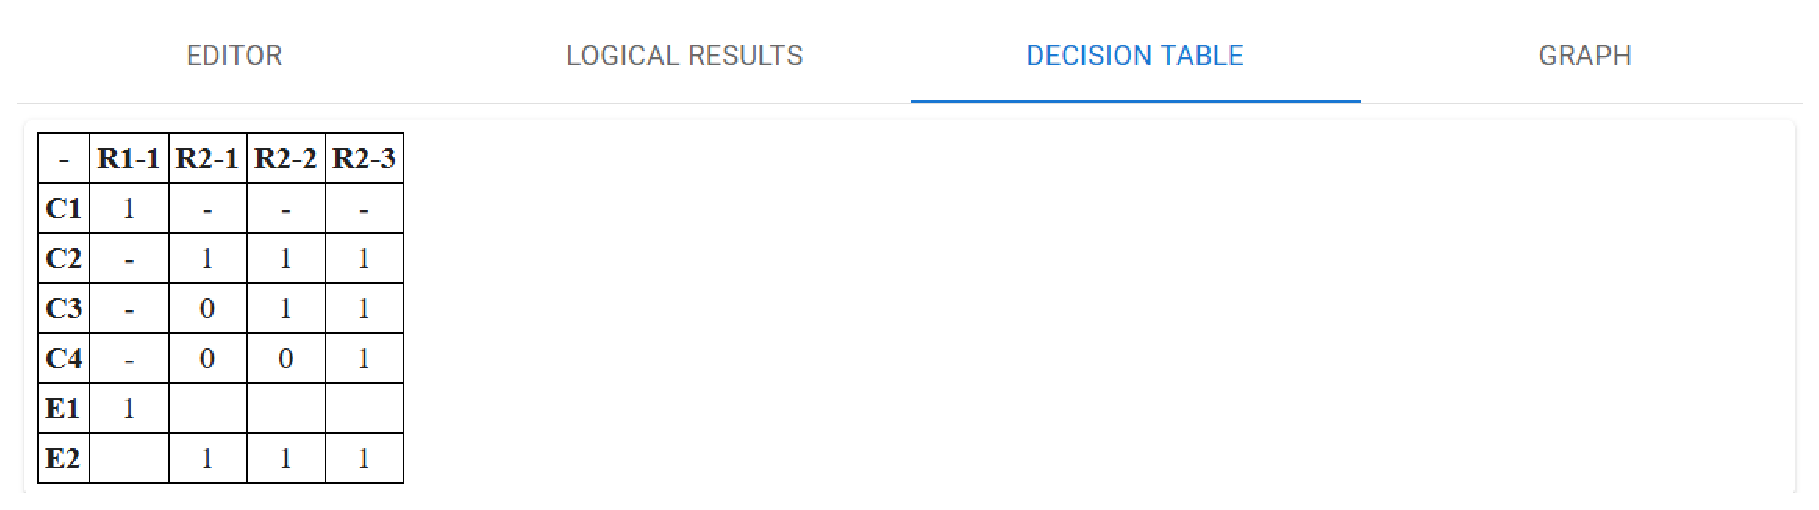
\includegraphics[width=0.8\textwidth,height=120px]{UIDecisionTable}
	\caption{User Interface - Decision Table tab}
	\label{fig:ui-decision-table}
\end{figure}

\subsection{Graph}

On the final tab, a visual representation of the defined graph is displayed. Each node, including causes, effects, and logical nodes, is represented in different colors for easy identification. The nodes are connected to one another by directed arrows, which serve as edges, clearly illustrating the relationships and flow between the various components of the graph.

\begin{figure}[H]
	\centering
	\includegraphics[width=0.8\textwidth,height=280px]{UIGraph}
	\caption{User Interface - Graph tab}
	\label{fig:ui-graph}
\end{figure}

\section{Kotlin Language Server}
\label{sec:kotlin-language-server}

To support client-side editing in the Monaco editor, a Kotlin Language Server connection was implemented. When the client editor initializes, it sends a connection request to the Back-End's socket interface. This interface is responsible for setting up and managing the connection between the client and the language server, allowing real-time code analysis, syntax highlighting, and other editor features to enhance the user experience.

Upon initialization, the Back-End starts the Kotlin Language Server as a child process. When a message arrives at the Back-End, it processes the message and then forwards it to the language server. Each response from the language server is similarly handled by the Back-End and relayed back to the client via the established Socket connection. This setup ensures smooth communication between the client editor and the language server, allowing for real-time feedback and interaction.

The syntax of the graph language has been integrated into the language server as an external library. This allows the language server to offer reliable assistance during editing, including features like code completion, syntax highlighting, and error detection, enhancing the overall user experience.

\begin{figure}[H]
	\centering
	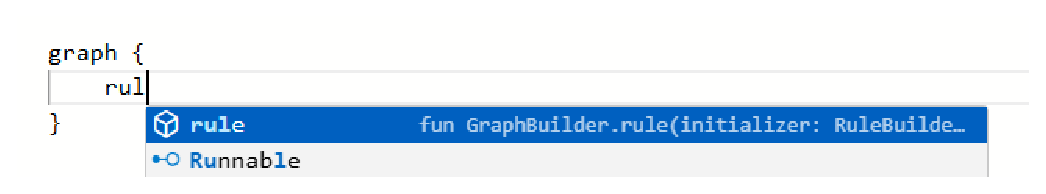
\includegraphics[width=0.8\textwidth,height=60px]{Intellisense}
	\caption{Monaco Editor intellisense for the graph language}
	\label{fig:editor-intellisense}
\end{figure}